

This chaper discuss the redundancy and scalability....
(2) Redundancy and Scalability:
We evaluated ECMP functionality by watching routing table updates on the router when the new load balancer is added or removed.
We also evaluated the performance level by changing the number of load balancers.

The following subsections explain the evaluation in detail.

%(3) Resource comsumption.
%We examined the basic performance of the our proposed load balancer container and the basic function of the ECMP redundancy using cluster of physical servers in on-premise data center.
%As for the performance, we measured throughput of the load balancer container and found that it was at least as good as existing software load balancer using Linux. 
%The ECMP redundancy is examined by . 
%We also demonstrate two different service with different number of load balancers can share the group of nodes.
%The portability of the load balancer is also evaluated using GCP and GCP.


\section{Redundancy and Scalability}

The ECMP technique is expected to make the load balancers redundant and scalable since all the load balancer containers act as active.
We examined the behavior of the ECMP routing table updates, by changing the number of the load balancers.
After that, in order to explore the scalability, we also measured the throughput from a benchmark client with ECMP routes when multiple of the ipvs container load balancers are deployed.

\begin{figure}[b]
    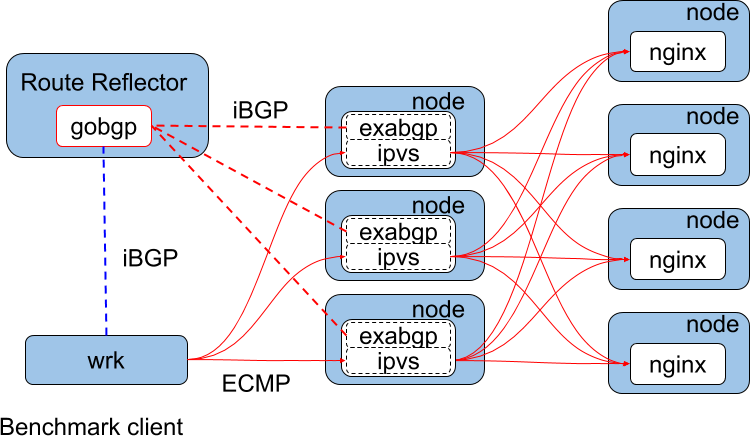
\includegraphics[width=0.9\columnwidth]{Figs/lb_ecmp_schem}
    \caption{}
    \label{fig:lb_ecmp_schem}
\end{figure}

\begin{table}[]
  \centering
  \begin{tabular}{ll}
    \hline \\
    \multicolumn{2}{l}{[Hardware Specification]}   \\
    & CPU: Xeon E5-2450 2.10GHz x 8 (with Hyper Threading) \\
    & Memory: 32GB \\
    & NIC: Broadcom BCM5720 Giga bit \\
    & (Node x 6, Client x 1) \\
    & \\
    & CPU: Xeon E5-2450 2.10GHz x 8 (with Hyper Threading) \\
    & Memory: 32GB \\
    & NIC: Intel X550 \\
    & (Load Balancer x 1) \\
    & \\
    \multicolumn{2}{l}{[Node Software]}  \\
    & OS: Debian 9.5, linux-4.16.8 \\
    & Kubernetes v1.5.2 \\
    & flannel v0.7.0 \\
    & etcd version: 3.0.15 \\
    & \\
    \multicolumn{2}{l}{[Container Software]}   \\
    & Keepalived: v1.3.2 (12/03,2016) \\
    & nginx : 1.15.4(web server) \\
    \\ \hline
  \end{tabular}
  \caption{}
  \label{tab:ecmp-hw_sw_spec}
\end{table}

Fig.~\ref{fig:ecmp-benchmark-schem} shows the schematic diagram of the experimental setup and also summarizes hardware and software specifications.
Notable differences from the previous throughput experiment in Fig.~\ref{fig:benchmark-schem} are as follows;
1) Each load balancer pods now consists of both an ipvs container and an exabgp container.
2) The routing table of the benchmark client is updated by BGP protocol through a route reflector.
3) The NIC of the benchmark client has been changed to 10 Gbps card since now we have multiple of ipvs container load balancers that are capable of filling up 1 Gbps bandwidth.
4) Some of the software have been updated to the most recent versions at the time of the experiment.


\begin{table}[h]

  \begin{subtable}{.9\textwidth}
  \centering
  \begin{tabular}{l}
    \hline 
    10.1.1.0/24 via 10.0.0.106 dev eth0 proto zebra metric 20 \\
    \hline
  \end{tabular}
  \caption{}
  \label{tab:single}
\end{subtable}

\begin{subtable}{.9\textwidth}
  \centering
  \begin{tabular}{ll}
    \hline
    \multicolumn{2}{l}{10.1.1.0/24 proto zebra metric 20 } \\
    \hspace{15 mm}
    & nexthop via 10.0.0.105  dev eth0 weight 1 \\
    & nexthop via 10.0.0.106  dev eth0 weight 1 \\
    & nexthop via 10.0.0.107  dev eth0 weight 1 \\
    \hline
  \end{tabular}
  \caption{}
  \label{tab:three}
\end{subtable}

\begin{subtable}{.9\textwidth}
  \centering
  \begin{tabular}{ll}
    \hline
    \multicolumn{2}{l}{10.1.1.0/24 pro to zebra metric 20 } \\
    \hspace{15 mm}
    & nexthop via 10.0.0.107  dev eth0 weight 1 \\
    & nexthop via 10.0.0.105  dev eth0 weight 1 \\
    & nexthop via 10.0.0.106  dev eth0 weight 1 \\
    \multicolumn{2}{l}{10.1.2.0/24 proto zebra metric 20 } \\
    \hspace{15 mm}
    & nexthop via 10.0.0.107  dev eth0 weight 1 \\
    & nexthop via 10.0.0.106  dev eth0 weight 1 \\
    \hline
  \end{tabular}
  \caption{}
  \label{tab:double_svc}
\end{subtable}

\caption{ECMP routing tables.}
\label{tab:exabgp_routing_table}
\end{table}

First, we examined ECMP functionality by watching the routing table on the benchmark client.
Table~\ref{tab:exabgp_routing_table}~(\subref{tab:single}) shows the routing table entry on the router when a single load balancer pod exists.
From this line, we can tell that packets toward 10.1.1.0/24 are forwarded to 10.0.0.106 where the load balancer pod is running.
It also shows that this routing rule is controlled by zebra.

When the number of the load balancer pods is increased to three, we can see the routing table entry in Table~\ref{tab:exabgp_routing_table}~(\subref{tab:three}).
We have three next hops towards 10.1.1.0/24 each of which being the node where the load balancer pods are running.
The weights of the three next-hops are all 1.
The update of the routing entry was almost instant as we increased the number of the load balancers.

Table~\ref{tab:exabgp_routing_table}~(\subref{tab:double_svc}) shows the case where we additionally started new service with two load balancer pods with service addresses in 10.1.2.0/24 range.
We could accommodate two different services with different IP addresses, one with three load balancers and the other with two load balancers on a group of nodes(10.0.0,105,10.0.0,106,10.0.0,107).
The update of the routing entry was almost instant as we started the load balancers for the second service.

\begin{figure}[t]
  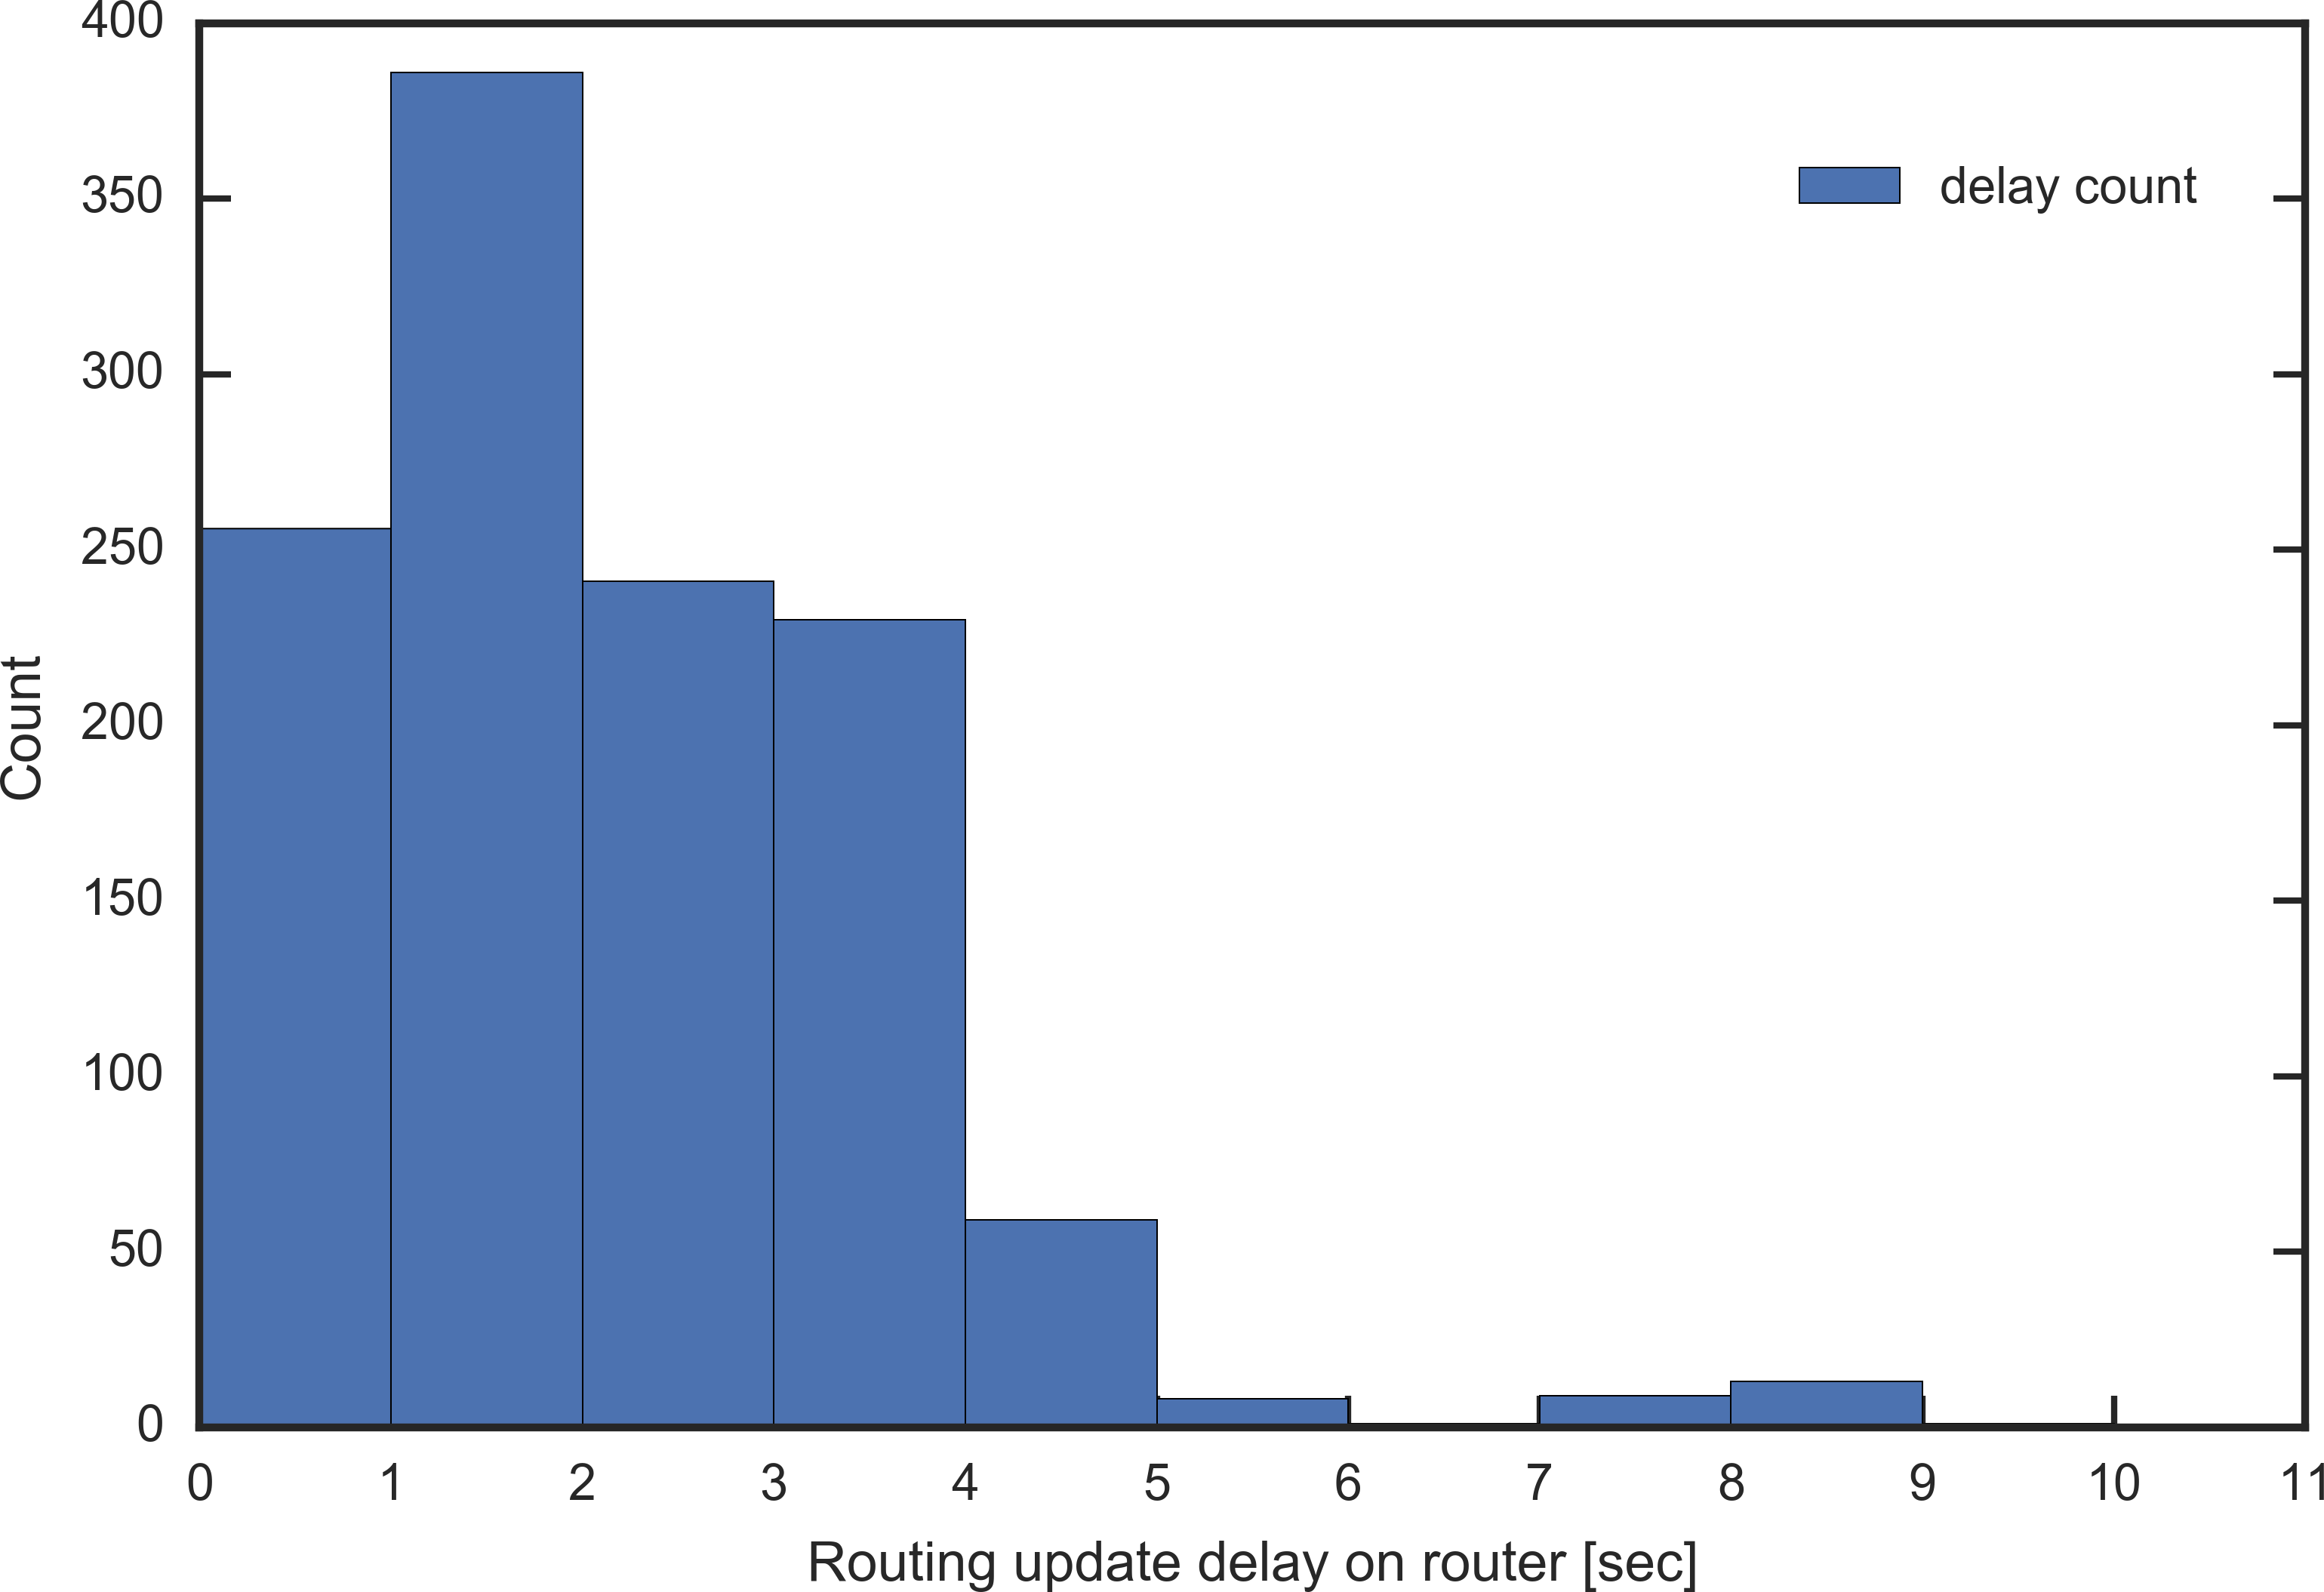
\includegraphics[width=0.9\columnwidth,left]{Figs/ecmp_delay_histgram}
  \caption{Caption 2}
  \label{fig:ecmp_delay_histgram}
\end{figure}

Fig.~\ref{fig:ecmp_delay_histgram} shows histogram of the ECMP update delay, where we measured the delays until the number of running ipvs pods is reflected in the routing table on the benchmark client, as we change the number of the ipvs pods randomly every 60 seconds for 20 hours.
As we can see from the figure, most of the delays are within 6 seconds, and the largest delay during the 20 hours experiment was 10 seconds.
We can conclude that ECMP routing update in our proposed architecture is quick enough.



We also carried out throughput measurement to show that our proposed architecture increases the throughput as we increase the number of the load balancers.
Fig.~\ref{fig:ecmp_lb_cubic} shows the results of the measurements.
There are four solid lines in the figure, each corresponding the throughput result when there are one through four of the proposed load balancers.
%As can be seen in the figure, as we increased the number of the pod the thoroughput increased linearly to a certain level after which it saturated.
The saturated levels, i.e. performance levels depend on the number of the ipvs load balancer pods(lb x 1 being the case with one ipvs pods, and lb x2 being two of them and as such), which increases linearly as we increases the number of the load balancers.
The dotted line in the figure shows the throughput result when there were five load balancers.
It had almost the same performance level as the case when there were four load balancers, and did not scale further.
We suspect that this was because we used up CPU power of the benchmark client since the CPU idle was 0\% when there were more than four load balancers.
We expect that replacing the benchmark client with more powerful machines, or changing the experimental setup so that multiple benchmark clients can access the load balancers through an ECMP router, will improve the performance level further.

Fig.~\ref{fig:ecmp_response} shows the throughput measurement results when we periodically changed the number of the load balancers. 
The red line in the figure shows the number of the ipvs load balancer pods, which we changed randomly every 60 seconds.
The blue line corresponds to the resulting throughput.
As we can see from the figure, the blue line nicely follows the shape of the red line.
This indicates that new load balancers are immediately utilized after they are created, and after removing some load balancers, the traffic to them is immediately directed to the existing load balancers.



\begin{figure}[t]
  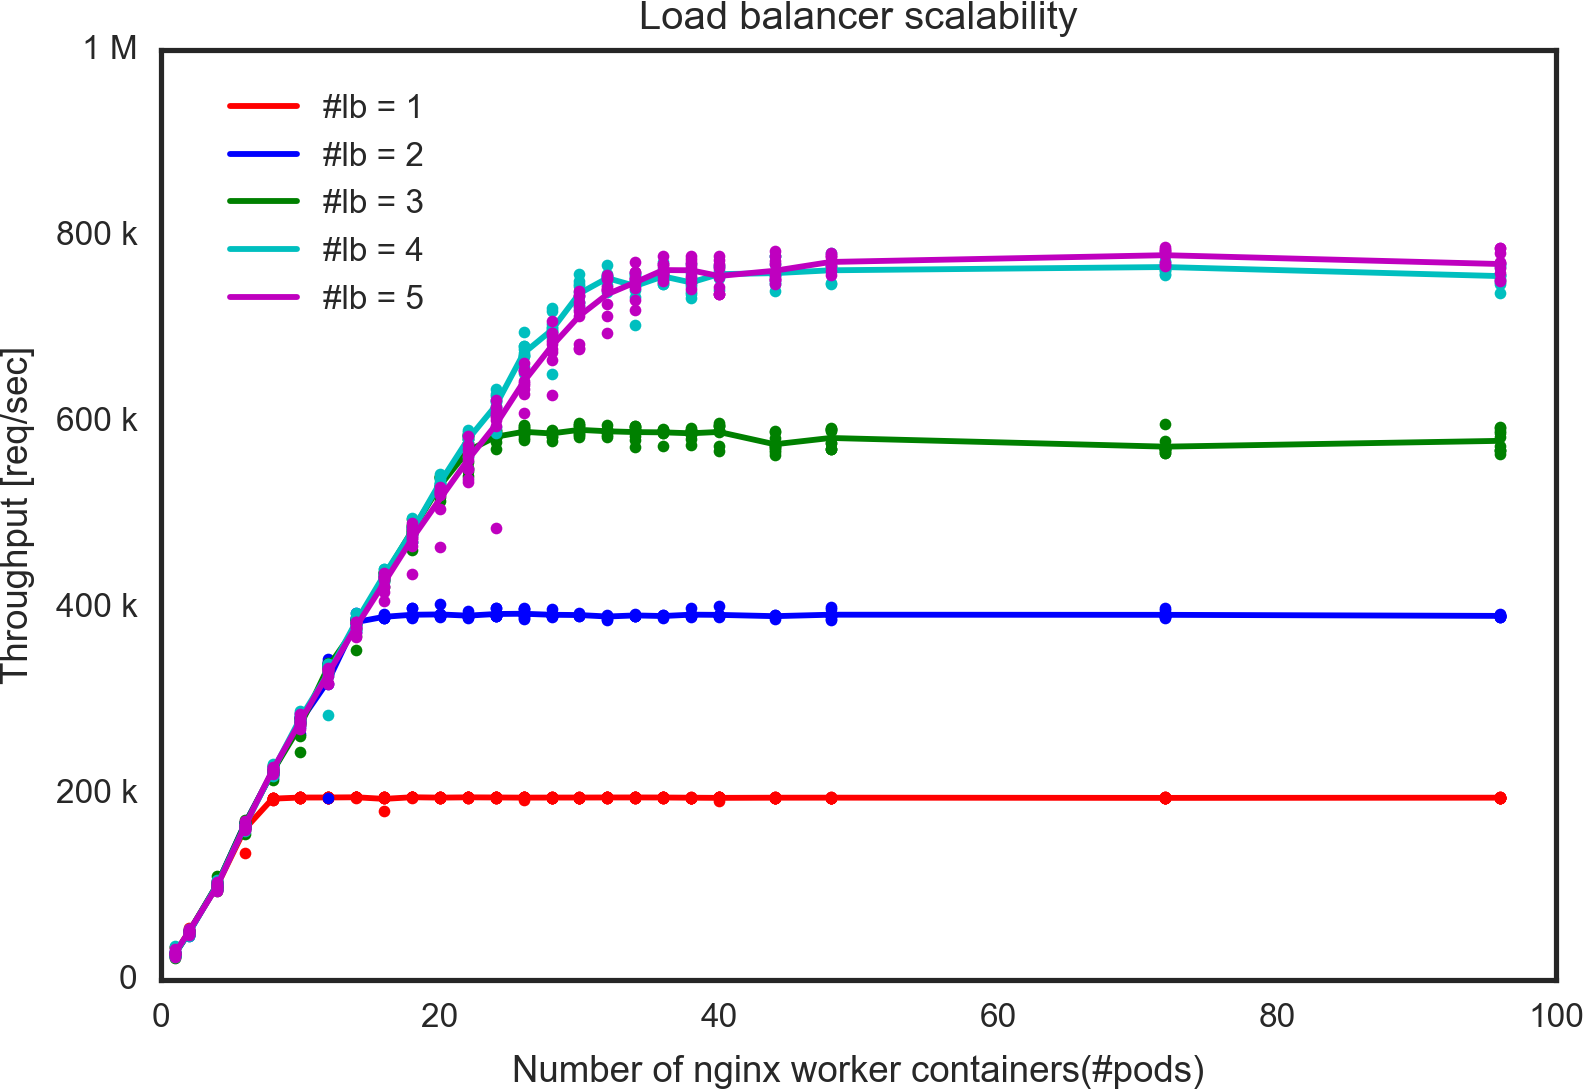
\includegraphics[width=0.9\columnwidth,left]{Figs/ecmp_lb_cubic}
  \caption{Caption 1}
  \label{fig:ecmp_lb_cubic}
\end{figure}

\begin{figure}[t]
  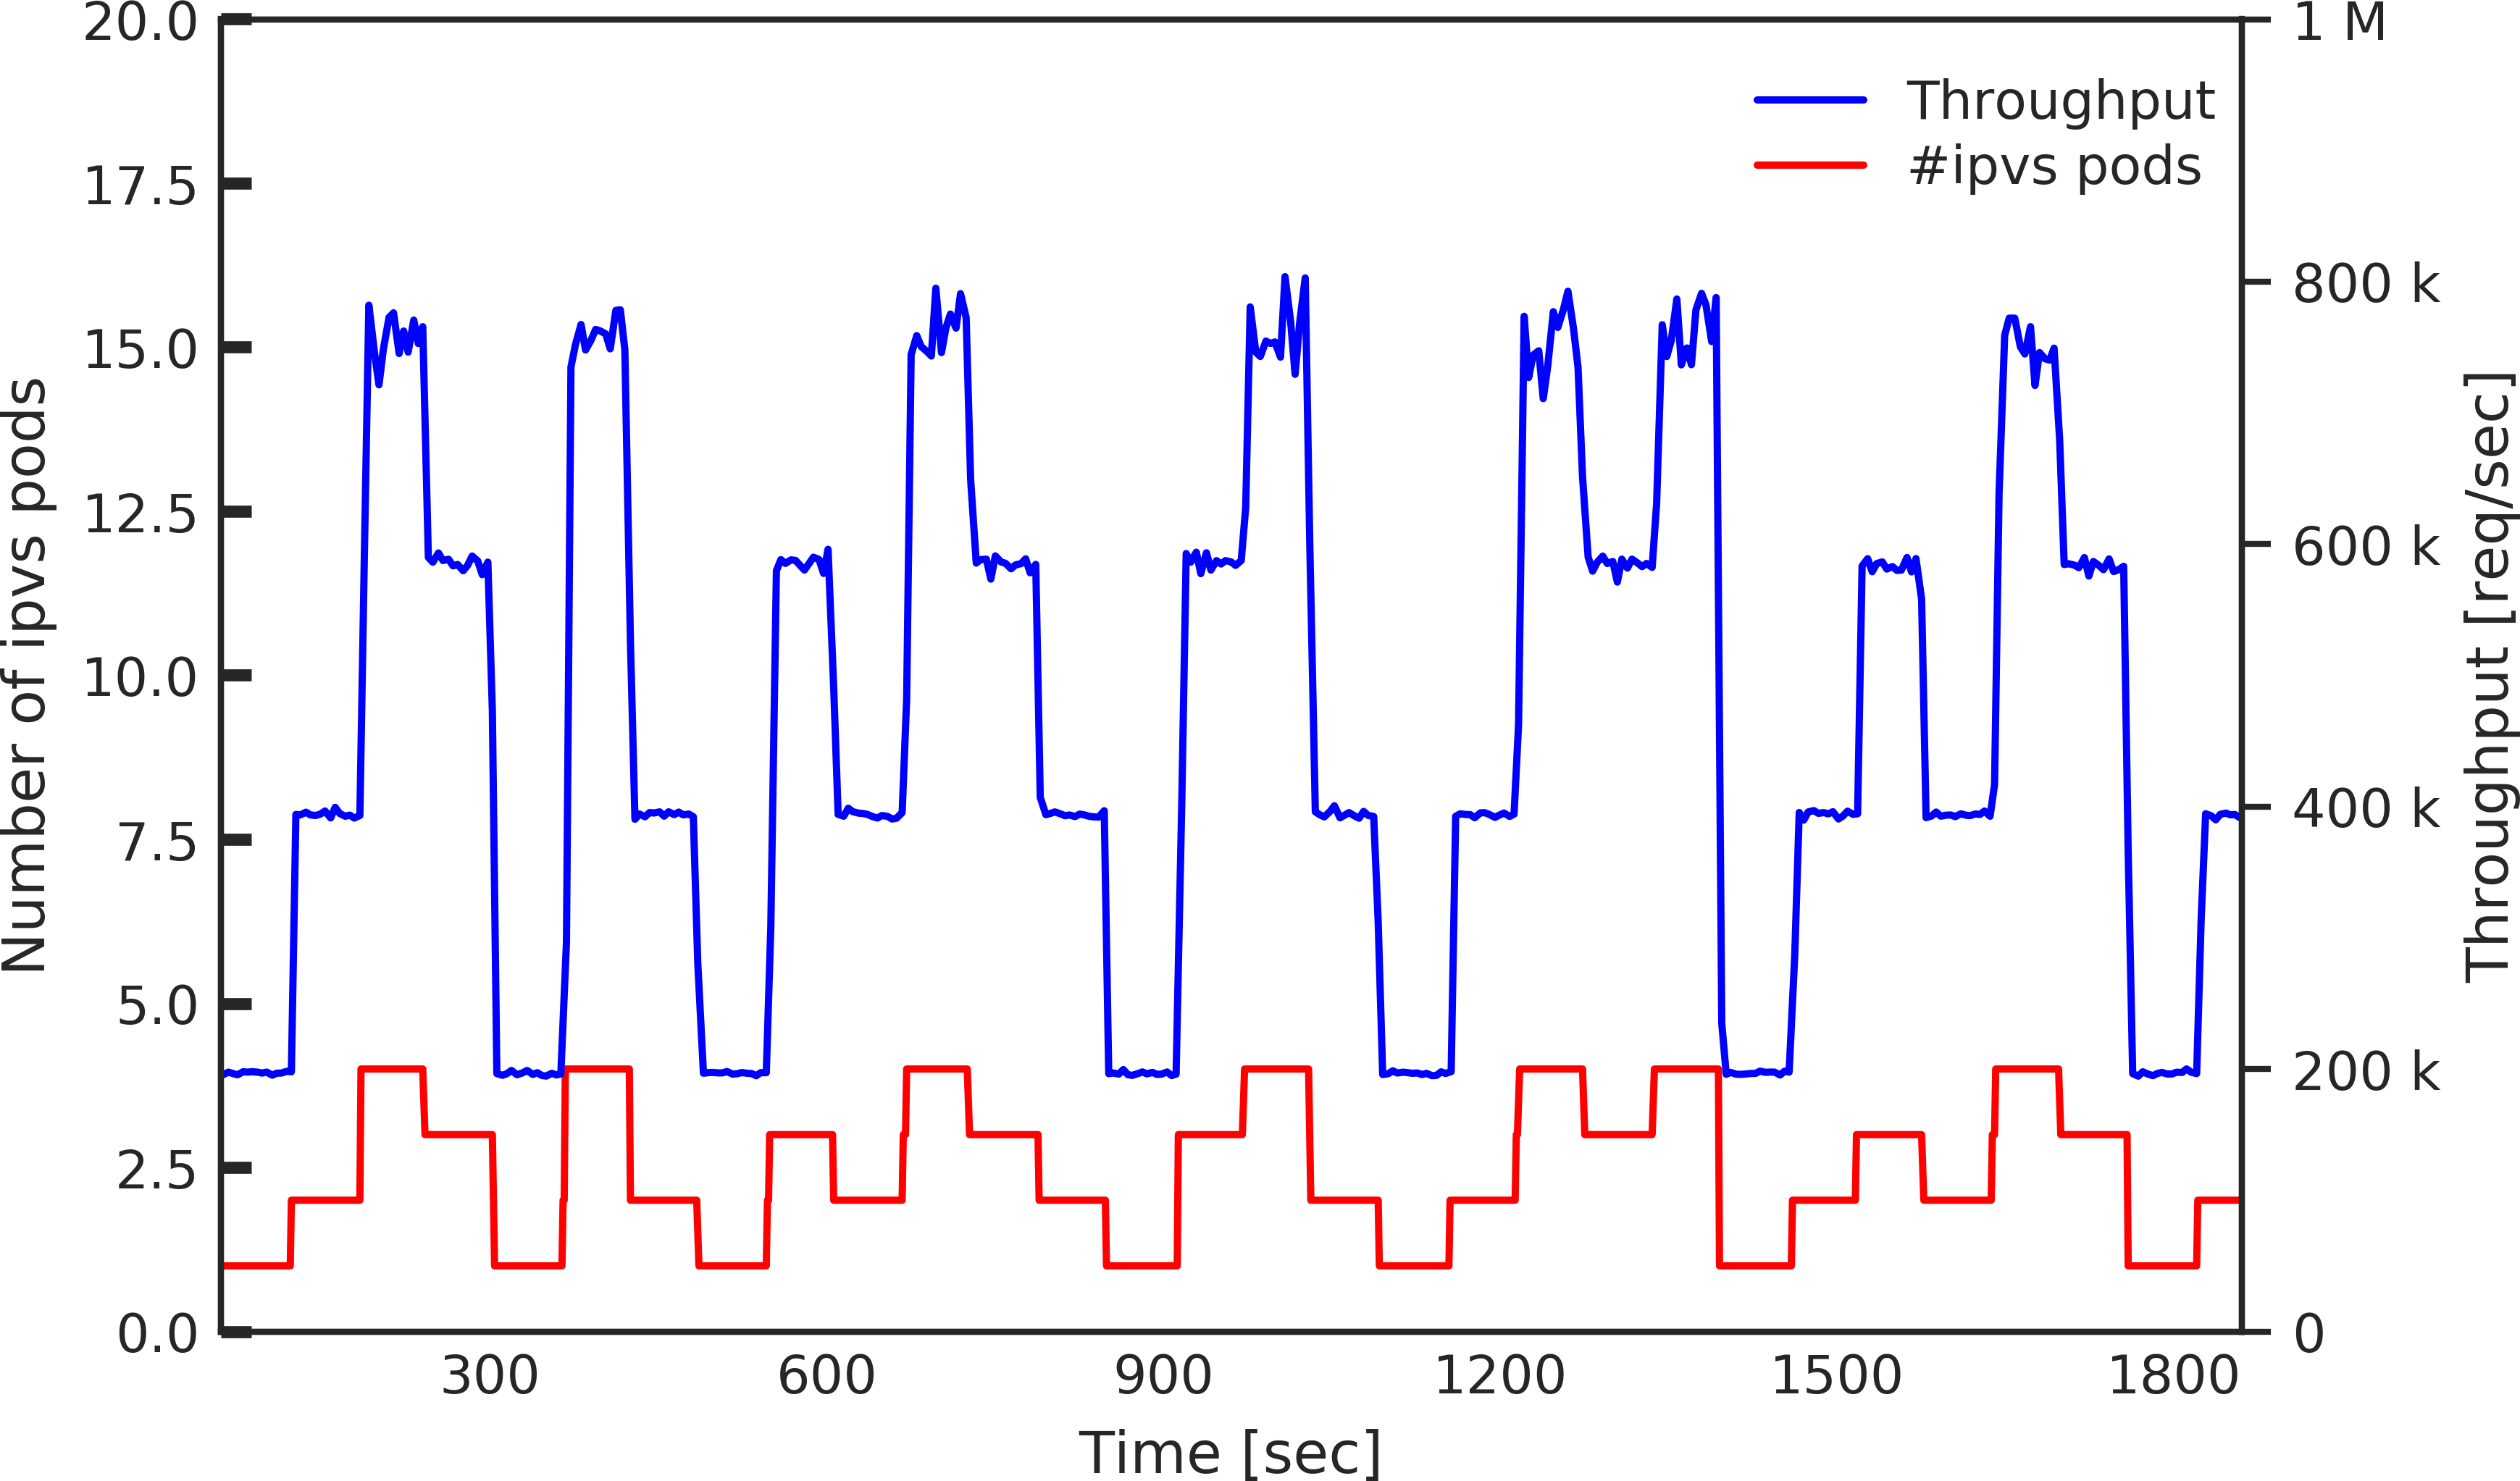
\includegraphics[width=0.98\columnwidth,left]{Figs/ecmp_response}
  \caption{Caption 2}
  \label{fig:ecmp_response}
\end{figure}


\section{Resource Consumption}



